\documentclass{article}
\usepackage{amsmath}
\usepackage{enumitem}
\usepackage{hyperref}
\usepackage{tikz}
\usepackage{pgfmath-xfp}
\usepackage{pgfplots}
\usepackage{pgfplotstable}

\begin{document}

\title{Course Outline: Regression Analysis}
\author{Muhammed Sezer \& Şevval Belkıs Dikkaya}
\date{}

\maketitle

\section{Introduction to Regression}

Regression analysis is a powerful statistical technique used to model the relationship between a dependent variable and one or more independent variables. It allows us to make predictions about the dependent variable based on the values of the independent variables.

In this course, we will cover the basics of regression analysis, including simple linear regression and multiple linear regression. We will also explore the assumptions and limitations of regression analysis, and learn how to interpret the results of a regression model.

By the end of this course, you will be able to build and interpret regression models, understand the strengths and limitations of regression analysis, and be able to apply these techniques to real-world problems. So, let's get started!

\subsection{Definition of Regression}

Regression analysis is a statistical method used to analyze the relationship between one or more independent variables and a dependent variable. It is used to predict the value of a dependent variable based on the value of one or more independent variables.

\subsection{Importance of Regression}

Regression analysis is important because it can help identify the strength and direction of the relationship between variables. This information can be used to make predictions and inform decision-making. Additionally, regression analysis can be used to test hypotheses about the relationship between variables.

\subsection{Brief History of Regression}

Regression analysis has a long history, with roots in the work of Francis Galton in the late 1800s. In the early 1900s, Karl Pearson developed the concept of correlation and expanded on Galton's work. In the 1930s, Ronald Fisher developed the method of least squares, which is still widely used in regression analysis today.

\subsection{Types of Problems that can be Solved using Regression Analysis}

Regression analysis can be used to solve a wide range of problems, including:

\begin{itemize}
\item Predictive modeling: predicting the value of a dependent variable based on the values of one or more independent variables
\item Causal inference: determining the causal relationship between variables
\item Forecasting: predicting future values of a dependent variable
\item Trend analysis: analyzing changes in a dependent variable over time
\item Quality control: identifying factors that contribute to variation in a dependent variable
\end{itemize}

\subsection{Applications of Regression in Various Fields}

Regression analysis is used in a variety of fields, including:

\begin{itemize}
\item Economics: analyzing the relationship between economic variables, such as GDP and unemployment
\item Finance: predicting stock prices based on market trends and other variables
\item Marketing: predicting consumer behavior based on demographic and behavioral variables
\item Healthcare: analyzing the relationship between patient characteristics and health outcomes
\item Education: predicting academic performance based on demographic and educational variables
\end{itemize}

Examples of specific applications of regression analysis include:

\begin{itemize}
\item Linear regression: predicting the price of a house based on its size, location, and other variables
\item Logistic regression: predicting whether a customer will churn based on their purchase history and other variables
\item Poisson regression: predicting the number of accidents on a given stretch of road based on traffic volume and other variables
\end{itemize}

\section{Theoretical Background of Regression}

In regression analysis, the goal is to estimate the relationship between a dependent variable ($Y$) and one or more independent variables ($X_1, X_2, ..., X_p$). This relationship is usually expressed as an equation, which is called the regression equation. The regression equation is used to predict the value of the dependent variable based on the values of the independent variables.

The general form of the regression equation is given as follows:

\begin{equation}
Y = f(X_1, X_2, ..., X_p) + \epsilon
\end{equation}

where $f(X_1, X_2, ..., X_p)$ is the functional form of the relationship between the dependent variable and the independent variables, and $\epsilon$ is the error term, which captures the random variation in the dependent variable that is not explained by the independent variables.

\subsection{Linear Regression Models and Assumptions}
Linear regression is a type of regression analysis that models the relationship between a dependent variable and one or more independent variables using a linear equation. The linear regression equation is given as follows:

\begin{equation}
Y = \beta_0 + \beta_1X_1 + \beta_2X_2 + ... + \beta_pX_p + \epsilon
\end{equation}

where $\beta_0$ is the intercept, $\beta_1, \beta_2, ..., \beta_p$ are the coefficients, and $X_1, X_2, ..., X_p$ are the independent variables.

The assumptions of linear regression models include:

\begin{itemize}
\item Linearity: The relationship between the dependent variable and the independent variables is linear.
\item Independence: The error terms are independent of each other.
\item Homoscedasticity: The variance of the error terms is constant across all levels of the independent variables.
\item Normality: The error terms are normally distributed.
\end{itemize}

\subsection{Polynomial Regression Models and Assumptions}
Polynomial regression is a type of regression analysis that models the relationship between a dependent variable and one or more independent variables using a polynomial equation. The polynomial regression equation is given as follows:

\begin{equation}
    Y = \beta_0 + \beta_1X_1 + \beta_2X_2 + ... + \beta_pX_p \\
    + \beta_{p+1}X_1^2 + \beta_{p+2}X_2^2 + ... + \beta_{2p}X_p^2 \\
    + \beta_{2p+1}X_1X_2 + ... + \beta_{(k-1)p+1}X_1^{k-1} + ... \\
    + \beta_{kp}X_p^{k-1} + \epsilon
    \end{equation}
    
    

where $\beta_0$ is the intercept, $\beta_1, \beta_2, ..., \beta_p$ are the coefficients of the first-order terms, $\beta_{p+1}, \beta_{p+2}, ..., \beta_{2p}$ are the coefficients of the second-order terms, $\beta_{2p+1}, ..., \beta_{(k-1)p+1}$ are the coefficients of the interaction terms, and $\beta_{kp}$ are the coefficients of the $k$th-order terms. $X_1, X_2, ..., X_p$ are the independent variables, and $\epsilon$ is the error term.

The assumptions of polynomial regression models are similar to those of linear regression models and include:

\begin{itemize}
\item Linearity: The relationship between the dependent variable and the independent variables is linear.
\item Independence: The error terms are independent of each other.
\item Homoscedasticity: The variance of the error terms is constant across all levels of the independent variables.
\item Normality: The error terms are normally distributed.
\end{itemize}

However, in polynomial regression models, the assumption of linearity requires that the relationship between the dependent variable and the independent variables be linear in terms of the transformed variables, not necessarily in terms of the original variables. Additionally, the assumption of independence applies to the error terms after the polynomial terms have been added to the model.


\subsection{Logistic Regression Models and Assumptions}
Logistic regression is a type of regression analysis used to model the relationship between a binary dependent variable and one or more independent variables using a logistic function. The logistic regression equation is given as follows:

\begin{equation}
p = \frac{1}{1 + e^{-(\beta_0 + \beta_1X_1 + \beta_2X_2 + ... + \beta_pX_p)}}
\end{equation}

where $\beta_0$ is the intercept, $\beta_1, \beta_2, ..., \beta_p$ are the coefficients, and $X_1, X_2, ..., X_p$ are the independent variables.

The logistic function is a sigmoidal function that ranges from 0 to 1, representing the probability of the dependent variable being in the "success" category. One advantage of logistic regression is that its derivative is easy to calculate and is defined, which is useful for optimization algorithms that require gradient information.

The assumptions of logistic regression models include:

\begin{itemize}
\item Independence: The observations are independent of each other.
\item Linearity of independent variables and log odds: The relationship between the independent variables and the log odds of the dependent variable is linear.
\item Absence of multicollinearity: The independent variables are not highly correlated with each other.
\item Large sample size: The sample size is large enough to ensure stable parameter estimates.
\end{itemize}

Note that normality and homoscedasticity are not assumptions of logistic regression models since the dependent variable is binary.

\subsection{Error Functions in Regression Models}

Error functions are used to measure the difference between the predicted values and the actual values in a regression model. The goal is to minimize this difference to obtain the best-fit line. There are several types of error functions, each with its own advantages and disadvantages. Here are some commonly used error functions in regression models:

\subsubsection{Mean Squared Error (MSE)}
\begin{center}
    \begin{tikzpicture}[scale=1.5]
    \draw[->] (-1.5,0) -- (1.5,0) node[right] {$y - \hat{y}$};
    \draw[->] (0,-0.5) -- (0,2) node[above] {$L$};
    \draw[scale=1,domain=-1.2:1.2,smooth,variable=\x,blue] plot ({\x},{\x*\x});
    \draw[dotted] (-1,1) -- (1,1);
    \draw[dotted] (1,0) -- (1,1);
    \draw[dotted] (-1,0) -- (-1,1);
    \node[left] at (0,1) {$MSE$};
    \node[below] at (1,0) {$\delta$};
    \node[below] at (-1,0) {$-\delta$};
    \end{tikzpicture}
    \end{center}
The mean squared error (MSE) is a commonly used error function in regression models. It measures the average of the squared differences between the predicted values and the actual values:

\begin{equation}
MSE = \frac{1}{n}\sum_{i=1}^{n}(y_i - \hat{y_i})^2
\end{equation}

where $n$ is the number of observations, $y_i$ is the actual value of the dependent variable for observation $i$, and $\hat{y_i}$ is the predicted value of the dependent variable for observation $i$.

The advantage of MSE is that it penalizes large errors more than small errors, making it useful in cases where we want to reduce the impact of outliers on the model.

\subsubsection{Mean Absolute Error (MAE)}
\begin{center}
    \begin{tikzpicture}[scale=1.5]
    \draw[->] (-1.5,0) -- (1.5,0) node[right] {$y - \hat{y}$};
    \draw[->] (0,-0.5) -- (0,2) node[above] {$L$};
    \draw[scale=1,domain=-1.2:1.2,smooth,variable=\x,blue] plot ({\x},{abs(\x)});
    \draw[dotted] (-1,1) -- (1,1);
    \draw[dotted] (1,0) -- (1,1);
    \draw[dotted] (-1,0) -- (-1,1);
    \node[left] at (0,1) {$MAE$};
    \node[below] at (1,0) {$\delta$};
    \node[below] at (-1,0) {$-\delta$};
    \end{tikzpicture}
    \end{center}
The mean absolute error (MAE) is another commonly used error function in regression models. It measures the average of the absolute differences between the predicted values and the actual values:

\begin{equation}
MAE = \frac{1}{n}\sum_{i=1}^{n}|y_i - \hat{y_i}|
\end{equation}

The advantage of MAE is that it is less sensitive to outliers than MSE, making it useful in cases where we want to reduce the impact of outliers on the model.

\subsubsection{Root Mean Squared Error (RMSE)}
\begin{center}
    \begin{tikzpicture}[scale=1.5]
    \draw[->] (-1.5,0) -- (1.5,0) node[right] {$y - \hat{y}$};
    \draw[->] (0,-0.5) -- (0,2) node[above] {$L$};
    \draw[scale=1,domain=-1.2:1.2,smooth,variable=\x,blue] plot ({\x},{sqrt(\x*\x)});
    \draw[dotted] (1,0) -- (1,1);
    \draw[dotted] (-1,0) -- (-1,1);
    \draw[dotted] (0,1) -- (1,1);
    \node[left] at (0,1) {$\sqrt{MSE}$};
    \node[below] at (1,0) {$\delta$};
    \node[below] at (-1,0) {$-\delta$};
    \end{tikzpicture}
    \end{center}
The root mean squared error (RMSE) is a variant of the MSE that takes the square root of the MSE. It is commonly used to measure the accuracy of a regression model:

\begin{equation}
RMSE = \sqrt{\frac{1}{n}\sum_{i=1}^{n}(y_i - \hat{y_i})^2}
\end{equation}

The advantage of RMSE is that it has the same units as the dependent variable, making it easier to interpret.

\subsubsection{R-squared}
\begin{center}
    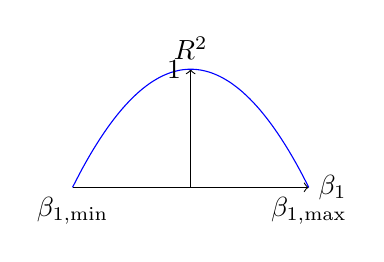
\begin{tikzpicture}[scale=1.5]
    \draw[->] (-1,0) -- (1,0) node[right] {$\beta_1$};
    \draw[->] (0,0) -- (0,1) node[above] {$R^2$};
    \draw[scale=1,domain=-1:1,smooth,variable=\x,blue] plot ({\x},{1-\x*\x});
    \node[below] at (1,0) {$\beta_{1, \text {max}}$};
    \node[below] at (-1,0) {$\beta_{1, \text {min}}$};
    \node[left] at (0,1) {$1$};
    \end{tikzpicture}
    \end{center}
    
R-squared is a statistical measure that represents the proportion of variance in the dependent variable that is explained by the independent variables in the regression model. It is also known as the coefficient of determination and is calculated as:

\begin{equation}
R^2 = 1 - \frac{SS_{res}}{SS_{tot}}
\end{equation}

where $SS_{res}$ is the sum of squared residuals, and $SS_{tot}$ is the total sum of squares.

The advantage of R-squared is that it provides a measure of how well the regression model fits the data, and it ranges from 0 to 1, with higher values indicating a better fit.

\subsubsection{Adjusted R-squared}
\begin{center}
    \begin{tikzpicture}[scale=1.5]
    \draw[->] (-1.5,0) -- (1.5,0) node[right] {$R^2_{adj}$};
    \draw[->] (0,-0.5) -- (0,2) node[above] {$p$};
    \draw[scale=1,domain=-1:1,smooth,variable=\x,blue] plot ({\x},{1 - \x*\x/2});
    \draw[dotted] (0,0) -- (0,1);
    \node[left] at (0,1) {$p_{max}$};
    \end{tikzpicture}
    \end{center}
Adjusted R-squared is a modified version of R-squared that adjusts for the number of independent variables in the model. It is calculated as:

\begin{equation}
Adjusted \ R^2 = 1 - \frac{(1 - R^2)(n - 1)}{n - p - 1}
\end{equation}

where $n$ is the number of observations, and $p$ is the number of independent variables.

The advantage of Adjusted R-squared is that it penalizes the inclusion of irrelevant variables in the model, making it a better measure of model fit.

\subsubsection{Akaike Information Criterion (AIC)}

Akaike Information Criterion (AIC) is a measure of the relative quality of a statistical model for a given set of data. It is calculated as:

\begin{equation}
AIC = -2ln(L) + 2p
\end{equation}

where $L$ is the likelihood of the data given the model, and $p$ is the number of parameters in the model.

The advantage of AIC is that it provides a measure of model quality that takes into account the complexity of the model.

\subsubsection{Mean Absolute Percentage Error (MAPE)}
\begin{center}
    \begin{tikzpicture}[scale=1.5]
    \draw[->] (-1.5,0) -- (1.5,0) node[right] {$y - \hat{y}$};
    \draw[->] (0,-0.5) -- (0,2) node[above] {$L$};
    \draw[scale=1,domain=-1.2:1.2,smooth,variable=\x,blue] plot ({\x},{abs(\x/1)});
    \draw[dotted] (-1,1) -- (1,1);
    \draw[dotted] (1,0) -- (1,1);
    \draw[dotted] (-1,0) -- (-1,1);
    \node[left] at (0,1) {MAPE};
    \node[below] at (1,0) {$\delta$};
    \node[below] at (-1,0) {$-\delta$};
    \end{tikzpicture}
    \end{center}
The mean absolute percentage error (MAPE) is an error function used in regression models to measure the average percentage difference between the predicted values and the actual values:

\begin{equation}
MAPE = \frac{1}{n}\sum_{i=1}^{n} \left| \frac{y_i - \hat{y_i}}{y_i} \right| \times 100%
\end{equation}

The advantage of MAPE is that it provides a measure of error in relative terms, which can be useful for comparing the performance of different models on different datasets.

\subsubsection{Mean Percentage Error (MPE)}
\begin{center}
    \begin{tikzpicture}[scale=1.5]
    \draw[->] (-1.5,0) -- (1.5,0) node[right] {$y - \hat{y}$};
    \draw[->] (0,-1.5) -- (0,1.5) node[above] {$L$};
    \draw[scale=1,domain=-1.2:1.2,smooth,variable=\x,blue] plot ({\x},{\x});
    \draw[dotted] (-1,-1) -- (1,1);
    \draw[dotted] (1,0) -- (1,1);
    \draw[dotted] (-1,0) -- (-1,-1);
    \node[left] at (0,1) {$100\%$};
    \node[right] at (0,-1) {$-100\%$};
    \node[below] at (1,0) {$\delta$};
    \node[below] at (-1,0) {$-\delta$};
    \end{tikzpicture}
    \end{center}
The mean percentage error (MPE) is another error function used in regression models to measure the average percentage difference between the predicted values and the actual values:

\begin{equation}
MPE = \frac{1}{n}\sum_{i=1}^{n} \left( \frac{y_i - \hat{y_i}}{y_i} \right) \times 100%
\end{equation}

The advantage of MPE is that it provides a measure of the direction of the error (i.e., overestimation or underestimation) in percentage terms.

\subsubsection{Mean Squared Log Error (MSLE)}
\begin{center}
    \begin{tikzpicture}[xscale=6]
    \draw[->] (0,0) -- (1,0) node[right] {$y - \hat{y}$};
    \draw[->] (0,0) -- (0,5) node[above] {$L$};
    \draw[scale=1,domain=0:1,smooth,variable=\x,blue] plot ({\x},{(ln(1)-ln(1+\x))^2});
    \node[left] at (0,5) {$MSLE$};
    \end{tikzpicture}
\end{center}


The mean squared log error (MSLE) is an error function used in regression models to measure the difference between the predicted values and the actual values in logarithmic space:

\begin{equation}
MSLE = \frac{1}{n}\sum_{i=1}^{n}(log(1+y_i) - log(1+\hat{y_i}))^2
\end{equation}

where $y_i$ is the actual value of the dependent variable for observation $i$, and $\hat{y_i}$ is the predicted value of the dependent variable for observation $i$.

The advantage of MSLE is that it penalizes underestimation and overestimation equally, making it useful in cases where both types of errors are equally important.

\end{document}